\documentclass[12pt,a4paper]{article}
\usepackage[utf8]{inputenc}
\usepackage[T1]{fontenc}
\usepackage{amsmath}
\usepackage{textcomp}

\usepackage{geometry}
\geometry{a4paper,left=25mm,right=25mm, top=2cm, bottom=2cm} 

\usepackage{graphicx} %fuer bilder

\usepackage{verbatim}




 \usepackage{mathptmx}
 \usepackage[scaled=.90]{helvet}
 \usepackage{courier}



\usepackage{listings}
\usepackage{color}
 
\definecolor{dkgreen}{rgb}{0,0.6,0}
\definecolor{gray}{rgb}{0.5,0.5,0.5}
\definecolor{mauve}{rgb}{0.58,0,0.82}

\pagestyle{empty}
\lstset{numbers=left, language=VHDL}
\lstset{showstringspaces=false,
basicstyle=\ttfamily\footnotesize,
breaklines=true,
tabsize=3,
commentstyle=\color{dkgreen},      % comment style
inputencoding={ansinew},
title=\lstname %zeigt titel der datei an
}

\usepackage{pdfpages} % fuer pdfs
\usepackage{hyperref} % fuer url


%keine einrückungen bei absatz
\parindent 0pt

\begin{document}
\title{Übung 04}
\author{Reinhard Penn, Bernhard Selymes, Robert Zeugswetter}
\date{Dezember 2015}

\normalsize


%Beginn des Dokuments

\newcommand{\Uebung}{ATPG}
\newcommand{\srcpath}{../../src}
\newcommand{\simpath}{../../sim}
\newcommand{\synpath}{../../syn}

%Angabe
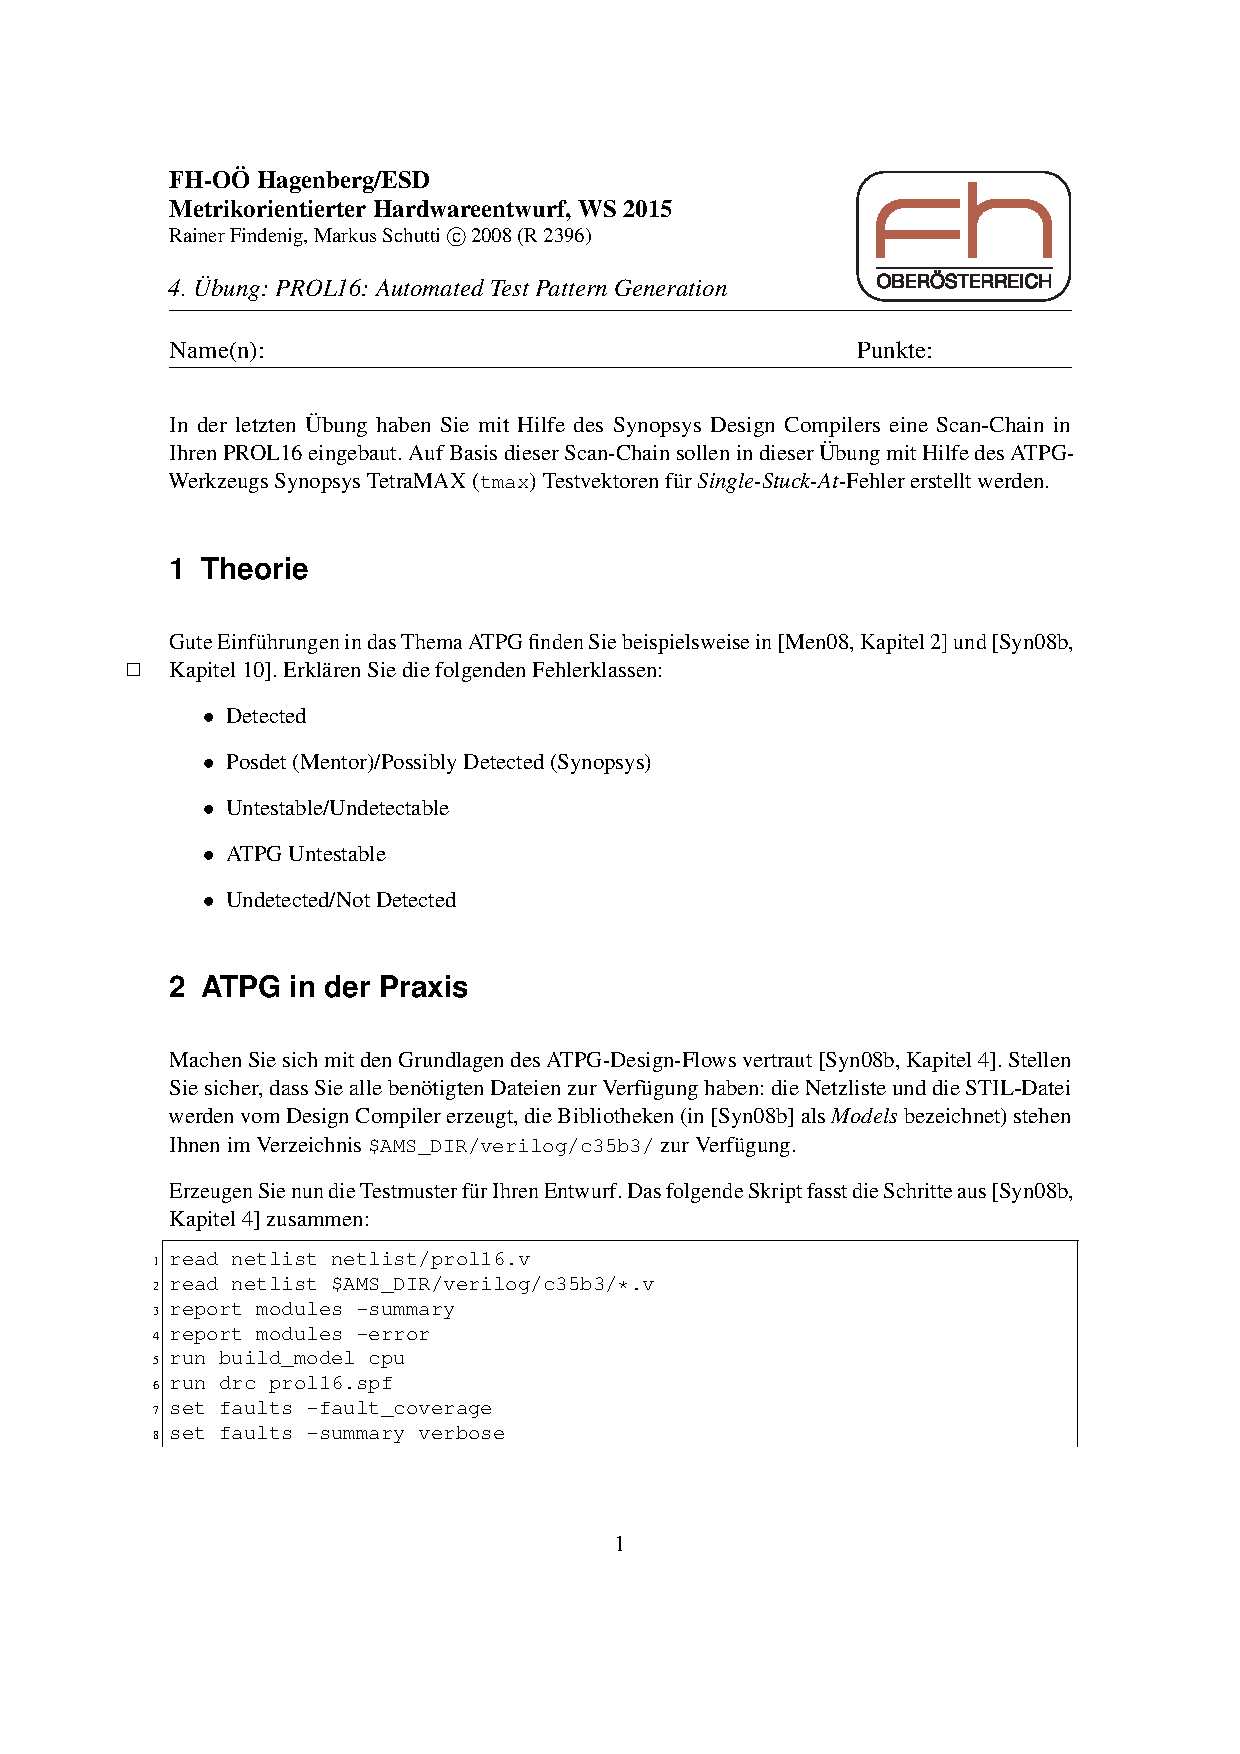
\includepdf[pages=-]{../Angabe.pdf}

\begin{center}
PROL16: Automated Test Pattern Generation\\
Übungsprotokoll zur Übung 4\\
Metrikorientierter Hardwareentwurf\\
Bernhard Selymes, Reinhard Penn, Robert Zeugswetter\\
07.12.2015
\end{center}

\section{Theorie}

Erklärung der Fehlerklassen:

\begin{itemize}

\item Detected\\
Diese Klasse inkludiert alle Faults die vom ATPG erkannt werden. Eine Subkategorie ist Detected by Simulation, hier 
werden Testpatterns generiert und anschließend simuliert um sicherzustellen das mit diesem Testpattern Faults erkannt werden.
Eine andere Subkategorie ist Detected by Implication. Faults dieser Art werden nicht von einem bestimmten Testpattern erkannt.
Sie treten in der Scankette auf, zum Beispiel beim Scanketteneingang oder beim Takt der Scankette.

\item Posdet\\ (Mentor)/Possibly Detected (Synopsys)
Diese Klasse ist in zwei Kategorien unterteilt. Die erste ist ATPG possibly detected. Hier sind alle Faults enthalten für die
nicht bekannt ist ob sie am fehlerhaften Gerät den Wert 0 oder 1 annehmen. Mithilfe einer Analyse ist bewiesen, dass der Fault
unter derzeitigen ATPG Bedingungen nicht zu 100\% erkannt werden kann. Die Kategorie not analyzed-possibly detected besagt das selbe
mit dem Unterschied das hier das Ergebniss der Analyse ob der Fault unter derzeitigen ATPG Bedingungen zu 100\% erkannt werden kann
inkonklusiv war.

\item Untestable/Undetectable\\
Faults in dieser Klasse können mit keinem Testpattern erkannt werden. Sie beinflussen allerdings auch das Verhalten des
Systems nicht. Eine mögliche Art von Untestable Faults sind die Unused Faults, ein Fault dieser Art kann auftreten wenn 
der Fault an einem offenen Ausgang auftritt. Im Vergleich dazu gibt es auch noch die Klasse Tied, Faults in dieser Klasse
treten auf Pins auf die auf einen bestimmten Wert gesetzt sind. Es kann zum Beispiel ein stuck-at-0 Fault auf einem Pin
der auf 0 hängt nicht erkannt werden. Andere mögliche Arten sind Blocked und Redundant Faults.

\item ATPG Untestable\\
Faults in dieser Klasse können mithilfe von ATPG nicht erkannt werden, aber sie können durch andere Methoden erkannt werden,
zum Beispiel funktionale Tests. Eine Art von Faults in dieser Klasse sind Faults von sequentiellen Elementen die nicht in der
Scankette sind, zum Beispiel Latches.

\item Undetected/Not Detected\\
Faults kommen in diese Klasse wenn die Analyse nicht abgeschlossen oder abgebrochen wurde. Ein möglicher Grund dafür,
ist das erreichen des ATPG Iterationslimit. Die zwei Subkategorien dieser Klasse sind not controlled und not observed.
Not controlled Faults treten auf wenn der ATPG Algorithmus keinen 1 oder 0 erzeugen kann und der Status immer auf X bleibt.
Not observed Faults treten auf wenn die Faults nicht in die Scankette oder an einen Ausgang weitergeleitet werden können.

\end{itemize}

\section{ATPG in der Praxis}

\subsection{Ergebnisse}
Die Ergebnisse der Simulation werden in der Datei in die unterschiedlichen Fehlerklassen unterteilt. Die test coverage ist naturgemäß größer als die fault coverage. Der Unterschied zwischen den beiden Werten kommt durch die undetectable faults zustande.
\lstinputlisting[language=c]{../atpg_results.rep}

\subsection{Coverage}
Beschreibung der Coverage-Werte laut TetraMAX® ATPG User Guide, Kapitel 10:
\begin{itemize}

\item Test Coverage\\
Test coverage gives the most meaningful measure of test pattern quality and is the default
coverage reported in the fault summary report. Test coverage is defined as the percentage
of detected faults out of detectable faults.

\item Fault Coverage\\
Fault coverage is defined as the percentage of detected faults out of all faults.
Fault coverage gives no credit for undetectable fault.

\end{itemize}

\newpage
\section{Simulation der Testmuster}

\subsection{Detected by Simulation}
Der Ausgang eines Nands in der ALU wird auf 0 gesetzt. Dieser Fehler führt zu vielen Fehlern in der Simulation.

\begin{lstlisting}
  //detectable error
  assign n148 = 0;
  NAND30 U211 ( .A(n152), .B(n150), .C(alu_func_i[3]), .Q() );
\end{lstlisting}

Ausgabe Simulation:
\begin{verbatim}
# DPV: End of STIL data; validation of 209 patterns FAILED 
with 343 output mismatches
\end{verbatim}

\subsection{Nicht-detektierbarer Fehler}
In der ALU der Prol16 ist ein Ausgangsport nicht verbunden. An diesen wird ein Stuck-At-1 Fehler angehängt. Dieser Fehler wird nicht erkannt in der Simulation.

\begin{lstlisting}
  alu_16_DW01_add_0 add_110 ( .A({n2, side_a_i, n1}), .B({n2, add_b, add_cin}), 
        .CI(n2), .SUM({res_v_17, res_v_16, res_v_15, res_v_14, res_v_13, 
        res_v_12, res_v_11, res_v_10, res_v_9, res_v_8, res_v_7, res_v_6, 
        res_v_5, res_v_4, res_v_3, res_v_2, res_v_1, SYNOPSYS_UNCONNECTED__0})
         );

  // undetectable error
  assign SYNOPSYS_UNCONNECTED__0 = 1;
\end{lstlisting}

Ausgabe Simulation:
\begin{verbatim}
# DPV: End of STIL data; validation of 209 patterns 
completed successfully with no errors
\end{verbatim}

\end{document}
